\section{实验结果}
\subsection{静态检查发现了什么，又遗漏了什么}
470条实际命令观察中，134条在受支持范围内静态一致，3条存在接口冲突，
333条为未知，未知比例为70.85\%。
三条冲突来自同一 \texttt{senior-ml-engineer} 包的文档示例：
示例使用的参数没有出现在相应脚本的字面解析器中，而脚本要求的必填参数又未被提供。
这能反驳特定示例的一致性，不能据此判定整个包在任何任务上都无效。
41个父包的95次本地资源提及未能按当前规则解析，涉及84个父包--目标路径组合；
其中可能包含示例和可选阅读，不作为确认缺陷计数。

\begin{table}[t]
\caption{受控接口干预结果。强标准库参照与扩展规则均达到当前受限机械契约的满检出；不能外推成整体质量准确率。}\label{tab:faults}
\centering\small
\begin{tabularx}{\columnwidth}{Xrrr}
\toprule
已知缺陷 & 数量 & 参数名规则 & 扩展/标准库 \\
\midrule
虚构选项 & 80 & 80 & 80/80 \\
遗漏必填 & 22 & 0 & 22/22 \\
非法枚举 & 38 & 0 & 38/38 \\
数值类型 & 14 & 0 & 14/14 \\
合计 & 154 & 80 & 154/154 \\
\bottomrule
\end{tabularx}
\end{table}

表\ref{tab:faults}给出已知干预的结果。
只检查参数名会漏掉74个必填、枚举和类型错误。
扩展检查与标准库参照均检出154个构造错误，在227个原始或无害对照上均无误报。
按35个父包平均，扩展检查的检出差为38.14个百分点，
条件重采样区间为29.88--46.00个百分点。
这是受限机械缺陷的诊断增量，不是超过标准库的新算法，也不是通用技能质量准确率。

在事后代码结构审查中，两个数据与机器学习技能包的六个方法主体只返回字面
\texttt{success=True}，并带有实现占位注释。
它们不能独自证明所声明业务已经完成，但整个包是否有其他实现路径仍未实测。
早期扫描还曾把行尾解释性注释作为命令参数，增加了11条错误线索；
修正词法处理后，线索从14条降为3条。
修正前源码与数据均保留，说明核验器本身也必须接受反例和语境复核。

\subsection{高定位有效率没有构成质量准确率}
\begin{table}[t]
\caption{真实模型评价先导。引用分母只来自结构合格响应，定位有效不代表语义支持。}\label{tab:judge}
\centering\small
\begin{tabularx}{\columnwidth}{Xrrr}
\toprule
提示 & 结构合格 & 引用定位 & 未知维度 \\
\midrule
普通rubric & 17/18 & 123/125 & 9/136 \\
支持证据优先 & 18/18 & 132/135 & 9/144 \\
反证优先 & 18/18 & 127/129 & 15/144 \\
\bottomrule
\end{tabularx}
\end{table}

54次真实评价中，53次通过结构检查。
普通rubric有一个响应同时给出“未知”状态和分值1，按预先规则记为不合格，未自动补值。
合格响应的389条引用中，382条通过严格定位，比例98.20\%。
表\ref{tab:judge}中三种提示的定位有效率相近，反证优先输出更多未知和冲突，
但没有独立语义金标准，不能判其更准确。
结构不合格响应的引用不进入定位比例，分母明确保留。

七条未通过定位的引用逐条复核后，四条是没有完整复制标注行的摘录，
三条指向目录中存在、但未放入编号正文的许可文件。
它们不能统称为虚构证据。
事后来源绑定器为全部389条引用取得了真实窗口：386条来自已提供的编号文档，
另三条由系统额外取回两个登记许可资源。
四条模型摘录差异仍保留，额外取证的来源也单列。
这验证的是可追溯窗口，不是389个语义判断正确。

\subsection{新产物实验：格式正确与计算正确明显分离}
\begin{table*}[t]
\caption{五臂实际产物结果。范围内每组48次；边界处置每组12次。费用只汇总范围内请求的峰价上界，不是独立账单。}\label{tab:execution}
\centering\small
\begin{tabularx}{\textwidth}{Xrrrrr}
\toprule
方法 & 合格数 & 成功率(\%) & 边界 & 平均输入token & 元上界 \\
\midrule
A0 无 Skill & 4/48 & 8.33 & 12/12 & 1706 & 0.2060 \\
A1 原始包 & 2/48 & 4.17 & 12/12 & 7122 & 0.7259 \\
A2 原包＋契约 & 4/48 & 8.33 & 12/12 & 7372 & 0.7500 \\
A3 无关上下文 & 6/48 & 12.50 & 12/12 & 5651 & 0.5847 \\
A4 仅契约 & 7/48 & 14.58 & 12/12 & 1955 & 0.2299 \\
\bottomrule
\end{tabularx}
\end{table*}

新实验完成全部300次请求，无基础设施错误、未运行或输出截断。
范围内五臂合计240份产物中只有23份完整通过，成功率为\NormalPassRate\%。
移除输入标识、哈希与额外字段等元数据约束后的数据指标合格数与主终点一致，
因此低成功率并非主要由形式字段导致。

表\ref{tab:execution}显示，原始包为2/48，无Skill和原包加契约均为4/48，
无关上下文为6/48，仅契约为7/48。
这些数值没有建立通用的优劣排序：只有一个目标技能，重复结果相关，输入是目的性构造，
无关上下文也没有精确匹配观测token。
特别地，无关上下文偶尔取得较高成功数，不能被解释为“不相关知识更好”，
而应提醒研究者避免从小样本排序直接推出方法胜负。

\begin{table*}[t]
\caption{预先固定的配对比较。差为百分点；区间是12个构造条件簇的条件重采样百分位区间，未经多重比较校正，不是总体保证。}\label{tab:effects}
\centering\small
\begin{tabularx}{\textwidth}{Xrrr}
\toprule
比较 & 均值差 & 95\%条件区间 & 胜/负/平 \\
\midrule
A1$-$A0 & -4.17 & [-14.58, 4.17] & 1/3/44 \\
A2$-$A1 & +4.17 & [-4.17, 12.50] & 3/1/44 \\
A4$-$A0 & +6.25 & [0.00, 12.50] & 3/0/45 \\
A2$-$A4 & -6.25 & [-12.50, 0.00] & 0/3/45 \\
A3$-$A0 & +4.17 & [0.00, 10.42] & 2/0/46 \\
\bottomrule
\end{tabularx}
\end{table*}

预先固定的条件簇比较见表\ref{tab:effects}。
原包加契约相对原始包的平均差为4.17个百分点，条件区间覆盖零；
仅契约相对无Skill的差为6.25个百分点，区间下界为零。
因此没有建立稳定的正向优势，更没有总体或跨模型保证。
仅契约的输入占用明显少于原始包，但它仍有41/48份范围内产物不合格，
不能仅凭较少token就认定已经得到可靠能力。

\begin{figure*}[t]
\centering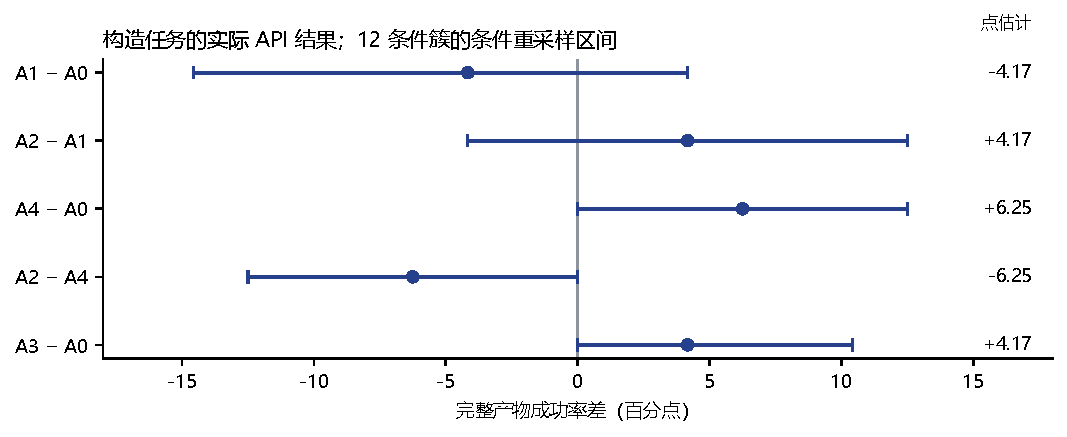
\includegraphics[width=.88\textwidth]{figures/paired_effects.pdf}
\caption{预先固定的五个配对比较。每个点来自实际API产物；线段为选定12个构造条件簇的95\%条件重采样区间，非标准误，也非技能总体的置信保证。图中颜色不编码显著性。}
\label{fig:effects}
\end{figure*}

\subsection{能力边界需要由失败层次刻画}
\begin{table}[t]
\caption{范围内输入规模分层。每个单元格为合格产物数/24次，两个重复不是独立任务。}\label{tab:sizes}
\centering\small
\begin{tabularx}{\columnwidth}{Xrr}
\toprule
方法 & 8行 & 48行 \\
\midrule
A0 无 Skill & 4/24 & 0/24 \\
A1 原始包 & 2/24 & 0/24 \\
A2 原包＋契约 & 4/24 & 0/24 \\
A3 无关上下文 & 6/24 & 0/24 \\
A4 仅契约 & 7/24 & 0/24 \\
\bottomrule
\end{tabularx}
\end{table}

六类明确元数据边界在五臂、两次重复下共60次处置全部合格。
与此同时，48行输入的120份范围内产物没有一份完整通过；
8行输入的120份产物只有23份合格（表\ref{tab:sizes}）。
边界处置和计算成功显然不能混成一个指标。
这些结果也不足以把8行认证为可靠能力区间，或把48行判定为绝对上限：
只观测了两个规模，且较小规模仍有较高失败率。

错误主要集中于过期记录计数：240份范围内产物中有216份在此项失败，
最大年龄错误20份、逐列空值错误10份、完整重复错误9份、行数错误4份。
这些错误计数可以重叠，不能相加后当作不同失败任务数。
即使温度为零，120个相同输入--方法的重复对中仍有7对的完整通过状态不同，
24对的产物数值不同；温度设定不是外部服务完全确定性的证明。

以一个8行普通CSV为例，基准日为2026-11-11，八条记录年龄依次为
$[7,1,31,8,31,7,1,0]$ 天，严格超过七天的记录应为3条。
同一输入的一次无Skill响应报告2条，原始包报告3条，而原包加契约报告0条。
其他字段可同时正确。
这一案例给出了可手工复核的失败机制，不能被引用定位或结构合格所弥补。

\subsection{事后测量诊断：平均检查掩盖完整任务失败}
这是在预定主分析之外进行的解释性诊断，不作为新的显著性检验。
每份范围内产物有9个输出字段及1个精确schema检查，共2,400项检查，
仅259项失败，平均检查通过率为\CheckPassRate\%。
即使只平均五个数据测量检查，通过率也有\MeasurePassRate\%，
但完整产物成功率仍仅\NormalPassRate\%。
该比例不是原项目既有质量分；它说明把多个容易条件与关键条件平均，
可以让同一批输出看起来远比实际可用程度好。

对同一批产物做发布门禁回放，全部接受会放行217份不合格产物；
全部拒绝虽无错误放行，但正确产物覆盖为零。
完整验收器门禁放行23份，按本构造真值没有错误放行。
后者是验收规则定义下的发布决定，不增加模型求解成功，也不是开放任务上的风险保证。
其价值在于显式呈现错误放行与覆盖，而非用全拒绝伪装优秀系统。

\subsection{网络侧：多样性没有自动形成完整能力覆盖}
\begin{table*}[t]
\caption{全库Fabric组的历史检索回放。既见12例不是新留出；相关性与完整集合覆盖分别计量。}\label{tab:routing}
\centering\small
\begin{tabularx}{\textwidth}{Xrrrr}
\toprule
方法 & 20例R@5 & 20例F & 既见12 R@5 & 既见12 F \\
\midrule
原顺序 & 80.00 & 55.00 & 78.47 & 58.33 \\
MMR .7 & 80.00 & 55.00 & 75.69 & 50.00 \\
原核DPP & 80.00 & 55.00 & 78.47 & 58.33 \\
残差DPP .5 & 80.00 & 55.00 & 78.47 & 58.33 \\
残差DPP 1 & 80.00 & 55.00 & 78.47 & 58.33 \\
查询覆盖 .5 & 80.83 & 55.00 & 78.47 & 50.00 \\
候选池上限 & 100.00 & 100.00 & 94.44 & 91.67 \\
\bottomrule
\end{tabularx}
\par\vspace{2pt}{\footnotesize R@5与F单位均为百分比；候选池上限使用参考标签作事后上界，不是实际选择器。}
\end{table*}

六种策略在全部192份捕获上产生1,152条选择记录。
表\ref{tab:routing}展示全库Fabric组，其余组别随数据一并提供。
基准20例中查询覆盖的平均召回从80.00\%升至80.83\%，
完整参考集合覆盖仍为55.00\%。
既见12例中，MMR的完整覆盖从58.33\%降至50.00\%，
查询覆盖也降至50.00\%；DPP类代理多数保持原结果。
这些结果不支持“增加多样性必然改善网络”的假设，也不能据此否定使用不同表示和训练模型的DSR。

基准20例的必要参考技能都在候选池中，但原前五只有55\%完整覆盖，
说明该组存在选择余地。
既见12例的池上限本身也不完整，未召回的参考能力无法靠重排补回。
由于任务均已使用、参考标签按技能名匹配且可能遗漏等价技能，
本文不把这组指标宣称为新的外部泛化或实际编排成功率。
